\documentclass[12pt, a4paper]{article}
% \usepackage[slantfont, boldfont]{xeCJK}
\usepackage{ulem}
\usepackage{amsmath}
\usepackage{booktabs}
\usepackage{colortbl}
% \usepackage[top = 1.0in, bottom = 1.0in, left = 1.0in, right = 1.0in]{geometry}
\usepackage{lipsum}
\usepackage{graphicx}
\usepackage{hyperref}
\usepackage{listings}
\usepackage{xcolor}

% \newcommand{\texttt}[1]{\texttt{\hyphenchar\font=\defaulthyphenchar #1}}
% \DeclareFontFamily{\encodingdefault}{\ttdefault}{\hyphenchar\font=`\-}
% \usepackage[htt]{hyphenat}
% \newcommand{\origttfamily}{}%
% \let\origttfamily=\ttfamily%
% \renewcommand{\ttfamily}{\origttfamily \hyphenchar\font=45\relax}
% \setCJKmainfont{SimSun}
% \setCJKmonofont{SimSun}

% \setmainfont[BoldFont={SimHei},ItalicFont={KaiTi}]{SimSun}
% \setsansfont[BoldFont=SimHei]{KaiTi}
% \setmonofont{NSimSun}

\setlength{\parskip}{0.5\baselineskip}
\setlength{\parindent}{2em}

\newcolumntype{Y}{>{\columncolor{red}}p{12pt}}
\newcolumntype{N}{>{\columncolor{white}}p{12pt}}
% \title{???}
% \author{???}


% \lstset{numbers=left,
% numberstyle=\tiny,
% keywordstyle=\color{blue!70}, commentstyle=\color{red!50!green!50!blue!50},
% frame=shadowbox,
% rulesepcolor=\color{red!20!green!20!blue!20}
% }

\lstset{
  % language=[ANSI]c,
  basicstyle=\ttfamily,
  % basicstyle=\small,
  numbers=left,
  keywordstyle=\color{blue},
  numberstyle={\tiny\color{lightgray}},
  stepnumber=1, %行号会逐行往上递增
  numbersep=5pt,
  commentstyle=\small\color{red},
  backgroundcolor=\color[rgb]{0.95,1.0,1.0},
  % showspaces=false,
  % showtabs=false,
  frame=shadowbox, framexleftmargin=5mm, rulesepcolor=\color{red!20!green!20!blue!20!},
% frame=single,
%  TABframe=single,
  tabsize=4,
  breaklines=tr,
  extendedchars=false %这一条命令可以解决代码跨页时,章节标题,页眉等汉字不显示的问题
}
			
\newcommand{\fullimage}[1]{
	\begin{flushleft}
		\includegraphics[width=\textwidth]{#1}
	\end{flushleft}
}

\newcommand{\pause}[0]{}


\title{Team Project (V): Large-Scale Multiple-Terminal Path Finding}
\author{asdfasdf}

\begin{document}

	\sloppypar

	\maketitle
	
	\tableofcontents
	\newpage
	
	\section{Problem Description}
	
		\begin{center}
			\textbf{Large-Scale Multiple-Terminal Path Finding}
		\end{center}
		
		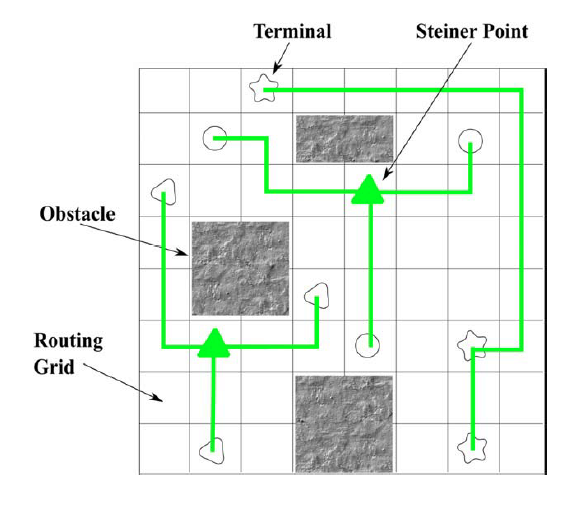
\includegraphics{problem.png}
		
		\begin{itemize}
		
		\item Given: $N \times N$ routing grids, and $M$ sets of terminals, where $N \geq 300, M \geq 10$ and each set has more than 3 terminals.
		\item Find: routing paths connecting each set of terminals.
		\item Constraints: different paths cannot cross each other, and no path can cross obstacles.
		\item Objective: (a) maximize the number of connected sets of terminals, and (b) when all sets of terminals can be connected,minimize the total length of all the paths.
		
		\end{itemize}
	
	\section{Overview}
	
<<<<<<< HEAD
		This document gives a method solving the problem decribed above. First, we give the overall design and system architecture of our project by giving the class design in the header file. Then, we introduce our algorithms which are used to solve this problem. Then, we give the OOP design of our project. Finally, we give the experiment results of this solving method.
=======
		This 
>>>>>>> a33bf05f9c0d3d34f6f0adf5f4e3b4923b14dfa9
	
	\section{Header Files and System Architecture}
	
		\subsection{Board.h}
		
			This class is used to describe the unsolved graph given by users. It has several attributes: height, width, the points in terminal sets which need to be connected, a map describing the points given by the users in the graph, and the points of blocks which the routes cannot go through. The board has two input methods: taking a set of points as input and taking a two-dimension array sized height $\times$ width. Both the two input methods will automatically generate the terminal sets and the map of the board. The output function is used to output the board.
		
		\subsection{TerminalSet.h}
		
			\texttt{TerminalSet} is the set of the terminal points which have the index. That is to say, the points with the same index will be in the same terminal set. \texttt{TerminalSet} has a \texttt{const Board} indicating which board it belongs to, a \texttt{vector} of points which are the terminal points, a \texttt{const int id} showing its index in the graph. Users can add points to this terminal set using \texttt{AddPoint} function.
				
		\subsection{Tree.h}

			\texttt{Tree} is a class which is used to describe one method connecting all the points in a terminal set. \texttt{map} is a \texttt{BitMatrix} used to describe the tree generated connecting this terminal set. \texttt{length} donates the total route-length of the tree and \texttt{computeLength()} is a function computing the length of the tree given the tree.
		
		\subsection{global.h}

			This file gives the definition of all the basic classes and the abbreviations used in this project. \texttt{Point} is the basic element of a graph represented by the position \texttt{x} and \texttt{y}. \texttt{Matrix} is a two-dimension \texttt{vector} which is used to store some value of the graph. \texttt{Vector} and \texttt{Pair} is inherited from STL and modification will be given if needed.
		
		\subsection{BitMatrix.h}

			\texttt{BitMatrix} is a bool matrix which is implemented to save memory, and also enabling fast copy and bitwise operations if needed.
		
		\subsection{Solution.h}

			As the name suggests, the \texttt{Solution} class is used to store the solution of the algorithm. It has a board given by the users given the original graph. \texttt{vector} trees is all the trees in the solution. \texttt{map} gives a graph of the solution which can be computed by the given trees using \texttt{computeMap()}.
		
		\subsection{Solver.h}
		
			This is the interface class for solving the problem. It only receives a \texttt{Board} and gives out a \texttt{Solution}. It will call the three strategies --- solve strategy, check strategy and optimize strategy in order to accomplish its function.
		
		\subsection{SolveStrategy.h}
		
			\texttt{SolveStrategy} is the interface class for giving a board and outputting a (primal) solution. The solution will be further optimized by other methods which is not cared about by this class.
			
			\texttt{CheckStrategy} provides the interface for checking the correctness of a solution, and \texttt{OptimizeStrategy} tries to optimize a solution.
		
		\subsection{StupidStrategy.h}
			
			This file implements three stupid strategies above: returing an empty solution, always returning legal, directly returning the original solution.
		
		\subsection{ColumnGenSolve.h}
		
			This class inherits \texttt{SolveStrategy} and implements the core (without divide-and-conquer) algorithm. The algorithm details will be discussed later.
		
		\subsection{CleverOptimize.h}
		
			This class create a new method optimizing the given solution. It inherits from the \texttt{OptimizeStrategy} and implements the optimize function. The concrete algorithm of this class will be discussed later in the algorithm part.
		
		\subsection{DACSolve.h}
		
			This class inherits \texttt{SolveStrategy} and implements the divide-and-conquer algorithm. The algorithm details will be discussed later.
		
		\subsection{test.h}
		
			This class provides a testing platform automatically calculating the running time of the test.
<<<<<<< HEAD

		\subsection{IntArray2bmp.h}

			This header file just gives a namespace that can be used to convert a two-dimension array to a picture.
=======
>>>>>>> a33bf05f9c0d3d34f6f0adf5f4e3b4923b14dfa9
		
		\subsection{GRBFactory.h}
		
			This class is the bridge between our project and Gurobi optimizer. It can configure the Gurobi enviroment and create enviroments for the project to use.
		
		\subsection{gurobi\_c++.h and gurobi\_c.h}
		
			These two files belongs to the Gurobi library.

	\section{Algorithm}
	
	\subsection{Column Generation}
	
	Let's assume we have found all Steiner trees connecting each set, then the problem can easily be formulated into a integer programming problem.
	
	Since generating all trees as well as integer programming problems are all difficult, we have to consider approximation. We can only consider the several ``best'' trees from each set, and both problems will be easy.
	
	We only need to define ``good'' trees and find them.
	
	First we construct the current best solution.
	
	For the sets in the solution, we regard other sets' trees in the solution as obstacles and try to reroute the current set.
	
	For each set, we run a new optimizing problem without the current set, and then regard other sets' trees in the solution to the new problem as obstacles and try to route the current set.
	
	We now only need a fast algorithm to route a set on a board with obstacles.
	
	The classic shortest Steiner tree algorithm needs $O(3^t n^2 + 2^t n^2 \log n)$ time, where $t$ is the number of terminals of the current set. It is OK with $t = 3, n = 300$ or like, but the algorithm is limited because it is unacceptable for any little larger $t$. In addition, it is no use to make the algorithm so precise in this step (since it is already a large approximation above).
	
	Our algorithm is based on Dijkstra's shortest path algorithm. We perform Dijkstra's algorithm from each terminal and enumerate the center. After connecting, the tree is not optimal usually (unless $t \leq 3$). We enumerate each edge and try to find another edge instead, where Dijkstra's algorithm is used again. We will stop optimize the tree when no possible edge can be improved.
	
	In addition, the Dijkstra results do not affect each other, so the algorithm is performed by multiple threads. Because our computing resource is limited, we only use two threads to boost the algorithm.
	
	When the solution is not improved after an iteration, the algorithm will terminate (though it is possible to improve if we do not terminate).
	
	\subsection{Divide and Conquer}
	
	Only using the algorithm above can get good results, but the divide-and-conquer strategy can improve the timing performance (though maybe decrease the solution quality a little).
	
	The strategy is simple. Divide the board into 4 parts as equal as possible. Solve the problem in each board. Assuming the points on trees of solution to the subproblems are all ``fixed'' terminals on the original board and do the final solve process.
	
	Thus, the solution space is more limited, and the running time will be improved. It is possible that the total number of the used grids may increase, but the number of connected sets will almost always improve.
	
	\subsection{CleverOptimize}
		
		This algorithm is used to optimize some solutions which are not good enough. Those which can be optimized will have the following attributes: the leaf of the tree can have a shorter route to the other routes of the tree. The algorithm implements as follows:
		
		Find the terminal set of the tree, go through every terminal of the tree and check each terminal point:
			
			Find the nearest point on the route which is connected to this point and has more than 3 degrees. Erase all the route between the terminal point and this point and again, find the shortest path from the terminal point to the left tree. This will guarantee the optimized route have the shorter length than the previous one. The process can be implemented by using simple bfs and backtrace. Note that if the found route which needs optimizing cross another terminal point, this route should not be optimized in case it makes another terminal point not connected to the route. If there is no point on the route having more than 3 degrees, we just put back the erased points to make sure the solution doesn't become worse. Implementing this algorithm has lots of incidents to consider about: the blocks which will be taken into account in the bfs process, the bfs process will also take the other terminal trees into account and this should not interfere the current route, etc.
	
	\section{OOP Design}
	
	\section{Experiment Results}

\begin{flushleft}
			\begin{tabular}{l l l l l l}
			\textbf{id} & \textbf{0} & \textbf{1} & \textbf{2} & \textbf{3} & \textbf{4} \\
			\midrule
			Size & 300 & 300 & 300 & 400 & 300 \\
			Set & 10 & 10 & 10 & 10 & 100 \\
			Terminal & 3 & 3 & 3 & 3 & 3 \\
			Block($*10^4$) & 0 & 1 & 2 & 1 & 1 \\
			Time  & 72.562s & 95.673s & 135.041s & 323.812s & 27m24.842s \\
			Connected Sets & 9 & 9 & 9 & 10 & 24 \\
			Length & 3490 & 3494 & 4060 & 6693 & 6693 \\
			\bottomrule
			\end{tabular}

			\begin{tabular}{l l l l l l}
			\textbf{id} & \textbf{5} & \textbf{6} & \textbf{7} & \textbf{8} & \textbf{9}\\
			\midrule
			Size & 300 & 300 & 300 & 350 & 350 \\
			Set & 30 & 10 & 10 & 10 & 10 \\
			Terminal & 3 & 5 & 10 & 3 & 5 \\
			Block($*10^4$) & 1 & 1 & 1 & 1 & 1 \\
			Time  & 25m8.331s & 90.156s & 736.371s & 159.130s & 258.372s  \\
			Connected Sets & 19 & 5 & 4 & 9 & 7  \\
			Length & 6783 & 2817 & 3735 & 4481 & 5387  \\
			\bottomrule
			\end{tabular}
\end{flushleft}

	
\end{document}






































